\section{Definition of Coordination Operators between the TFSM and Activity Language}
This section presents the \bcool specification of two coordination patterns between the TFSM and Activity languages. The specification relies on two operators named \emph{startActivityWhenEnter} and \emph{AtomicActivity}. These operators are used to capture a hierarchical and timing coordination pattern between states and activities. In the following, we present the \bcool specification of each operator.    


The \emph{startActivityWhenEnter} coordinates the entering and leaving of a state with the execution of an activity. The entering into a state is identified by the \textit{entering} \dse defined in the context of State. Instances of such \dse have to be coordinated with instances of the \textit{startActivity} \dse. Similarly, leaving a state is identified by \dse \textit{leaving} and finishing an activity is identified by \dse \textit{finishActivity}. 

\begin{lstlisting}[language=bcool,
caption={Hierarchical operator between TFSM and Activity languages},
label={lst:bcoolStartActivityWhenEnter}, 
basicstyle=\scriptsize\ttfamily, backgroundcolor=\color{LGrey}, numbers=left, xleftmargin=2pt]
Operator  StartActivityWhenEnter (activityStart : ad::startActivity , activityStop : ad::finishActivity, enterState : tfsm::entering, leaveState : tfsm::leaving)
when ((activityStart.name = activityStop.name ) and (enterState.name = leaveState.name) and (activityStart.name = enterState.onEnterAction.name));
do 
LoopFromStartToFinishNonPeemptive (enterState, leaveState, activityStart, activityStop)
end operator;
\end{lstlisting}

We use \bcool to define the operator \emph{startActivityWhenEnter} that has as parameters the \dse \textit{startActivity}, \textit{finishActivity}, \textit{entering} and \textit{leaving} (Listing~\ref{lst:bcoolStartActivityWhenEnter}: line 1). The operator selects instances of \dse \emph{startActivity} and \emph{finishActivity} by using their context (Listing~\ref{lst:bcoolStartActivityWhenEnter}: line 2). The pairs selected identify the starting and finishing of an activity. Then, we select the activities that represent a state by relying on the method \emph{onEnterAction} that is defined in the context of State. This method contains the name of the activity that the state represents (Listing~\ref{lst:bcoolStartActivityWhenEnter}: line 2). To coordinate the selected instances of \dse, we rely on the event relation \emph{LoopFromStartToFinishNonPeemptive} which makes the internal activity executes in a loop until the state is left. 


\begin{figure}
	\center
	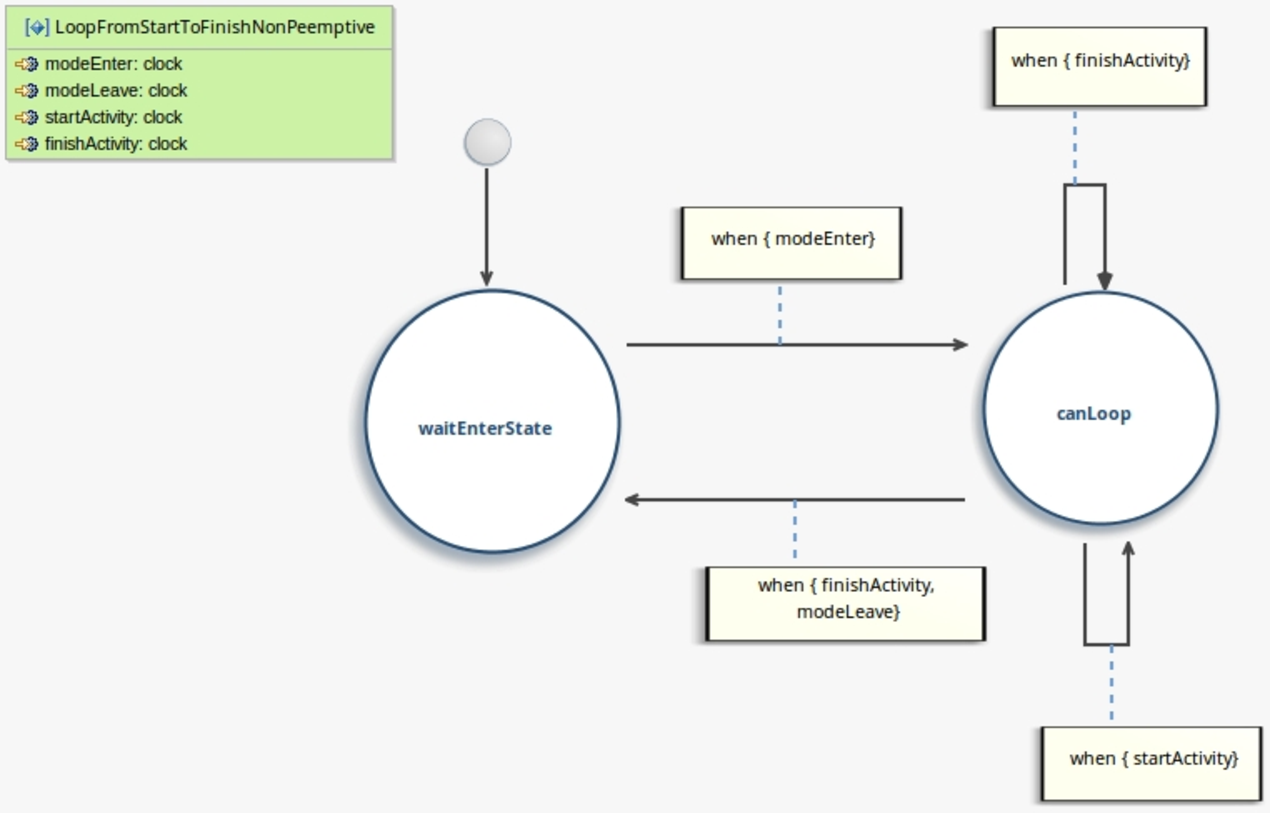
\includegraphics[width=.7\columnwidth]{examples/figs/LoopFromStartToFinishNonPreemptive}
	\caption{\emph{LoopFromStartToFinishNonPeemptive} event relation}
	\label{fig:looprelation}
\end{figure}

To specify the relation LoopFromStartToFinishNonPeemptive, we use \moccml to define an state-based relation (see Figure~\ref{fig:looprelation}). The relation takes four events as parameters: the events \emph{modeEnter} and \emph{modeLeave} that represents respectively the entering and leaving of a state; and the events \emph{startActivity} and \emph{finishActivity} that represents respectively the starting and finishing of an activity. The state-based representation is made of two states named \emph{waitEnterState} and \emph{canLoop}. In waitEnterState state, only the event modeEnter is allowed to tick and the activity is forbidden to execute. When the event modeEnter happens, the state \emph{canLoop} is reached and the events startActivity and finishActivity are allowed to occur, thus making the activity to execute in a loop. Only when the event modeLeave and finishActivivity happens simultaneously, the state can be left and the activity stops to execute. 

The use of this relation in the coordination rule results in a coordination in which the transitions in the TFSM cannot preempt the execution of the internal activities. The entering a state makes the activity to execute in a loop. Then, only after the activity has finished, the state can be left.


Similar than the \emph{startActivityWhenEnter} operator, the \emph{AtomicActivity} operator also defines a coordination between states and activities, but in this case, it deals with the temporal aspects of the coordination. The operator specifies how the time in the TFSM elapses during the execution of the activities that specify the on-entry action of a state. Thus, this coordination is also hierarchical, but in this case, only considers the timing aspects. %In these languages, the time is represented differently. In the TFSM language, each state machine has a \emph{localClock} used to measure the time while the Activity language is untimed. The local clock is a \emph{FSMClock}, which defines a \dse named \emph{ticks} whose occurrences represent a physical time increment. In the Activity language, the duration of activities can be represented as the time between the \dse \emph{startActivity} and \dse \emph{finishActivity}. Thus, to coordinate the time, it is necessary to specify the number of \emph{ticks} of the local clock between the occurrence of the \dse \emph{startActivity} and \emph{finishActivity}. In this operator, we propose to enforce the execution of the ``internal'' activity to be atomic with respect to the time in the TFSM model. As a result, there is no occurrence of the \dse ticks of the corresponding local clock during the execution of the activity. 

\begin{lstlisting}[language=bcool,
caption={Timing Hierarchical operator between TFSM and Activity languages},
label={lst:bcoolAtomicExec}, 
basicstyle=\scriptsize\ttfamily, backgroundcolor=\color{LGrey}, numbers=left, xleftmargin=2pt, firstnumber=6]
Operator AtomicActivity (activityStart : ad::startActivity , activityStop : ad::finishActivity, enterState : tfsm::entering, leaveState : tfsm::leaving, timeTicks : tfsm::ticks)
when ((activityStart.name = activityStop.name ) and (activityStart.name=enterState.OnEnterAction.name ) and (enterState.owningFSM.localClock = timeTicks));
do 
AtomicExec (activityStart, activityStop, timeTicks)
end operator;
\end{lstlisting}

In \bcool, we define the operator \emph{AtomicActivity} (Listing~\ref{lst:bcoolAtomicExec}: line 6) that specifies how time is consumed during the execution of the activities that are represented by states. The matching correspondence is similar that the previous operator: it selects instances of \dse \emph{startActivity} and \emph{finishActivity} by using their context and the onEnterAction is used to select the activities that represents a state. In addition, the matching correspondence selects instances of \dse ticks by relying on instances of \dse entering (Listing~\ref{lst:bcoolStartActivityWhenEnter}: line 7). To do so, we query the context of \dse \emph{entering} to get the localClock of the \emph{owningFSM} and then, we compare with the context of the \dse ticks. As a result, the selected instances of \dse ticks corresponds with the localClock of the TFSM that contains the state represented by the activity. 

\begin{figure}
	\center
	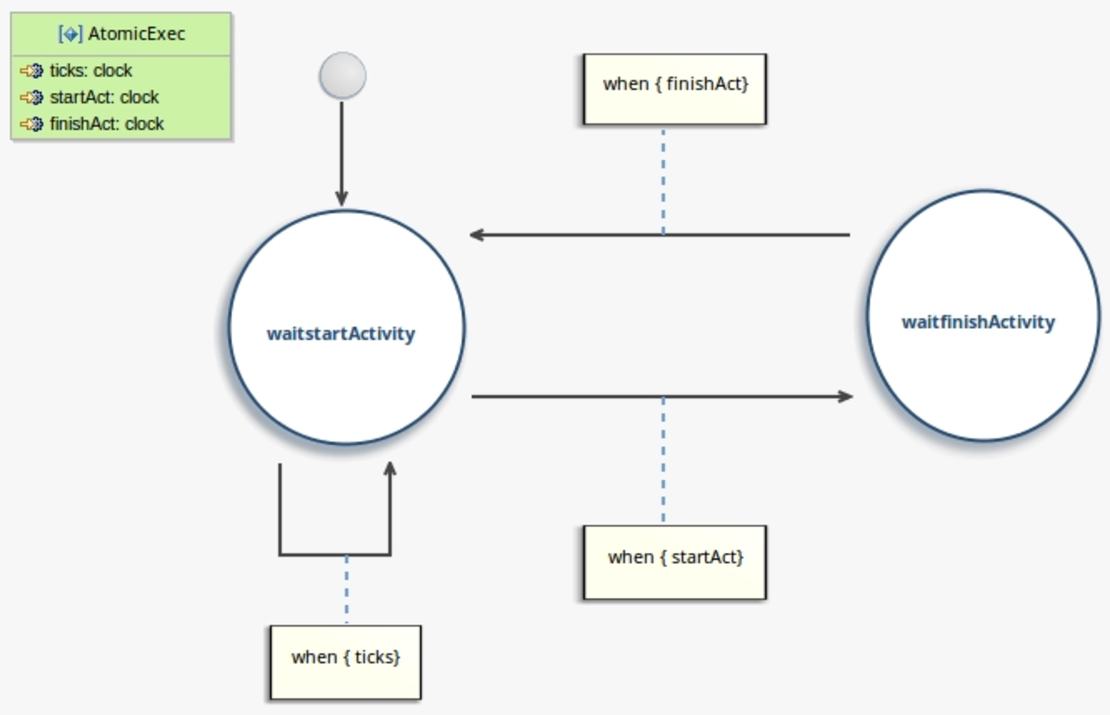
\includegraphics[width=.7\columnwidth]{examples/figs/AtomicExec}
	\caption{\emph{AtomicActivity} event relation}
	\label{fig:atomicexec}
\end{figure}

To express the coordination rule, we rely on the event relation \emph{AtomicExec} which makes the execution of the activities atomic with respect to the local clock of the TFSM. We specify this relation in \moccml (see Figure~\ref{fig:atomicexec}). The event relation accepts three events as parameters: \emph{ticks}, \emph{startAct} and \emph{finishAct}. While the event ticks represents the ticking of the local clock, the startAct and finishAct events represent respectively the starting and finishing of an activity. The state-based representation of the event relation is made of two states named \emph{waitstartActivity} and \emph{waitfinishActivity}. In \emph{waitstartActivity} state, the event ticks is allowed to occur, thus making the time elapse. When the startAct event happens, the \emph{waitfinishActivity} state is reached and the event ticks is forbidden to occur, \ie the time in the TFSM does not elapse while the activity executes. Only when the event finishAct happens, the \emph{waitstartActivity} state is reached, and \emph{ticks} is allowed to occur again. In the operator, we use this relation to make the execution of the activities atomic, \ie there is no occurrence of the \dse ticks of the corresponding local clock during the execution of the activity.

In this section, we have used \bcool to define a set of coordination operators that deal with both control and timing aspects of the coordination between states and activities. Unlike hierarchical coordination frameworks where the semantics is hidden, these operators explicitly specified how the hierarchical coordination is implemented. Together with the operator \emph{SyncFSMEventsAndActions} (Listing~\ref{lst:bcoolrunningexample}), in the next section, we use these operators to coordinate the models of the surveillance camera system.







